
\newtoggle{inTableHeader}% Track if still in header of table
\toggletrue{inTableHeader}% Set initial value
\newcommand*{\StartTableHeader}{\global\toggletrue{inTableHeader}}%
\newcommand*{\EndTableHeader}{\global\togglefalse{inTableHeader}}%

% Redefine tabular to initialize \StartTableHeader at start and end
\let\OldTabular\tabular%
\let\OldEndTabular\endtabular%
\renewenvironment{tabular}{\StartTableHeader\OldTabular}{\OldEndTabular\StartTableHeader}%

 %The min, mid and max values
\newcommand*{\MinNumberA}{0.5}%
\newcommand*{\MidNumberA}{0.75}%
\newcommand*{\MaxNumberA}{1.0}%

%Apply the gradient macro
\newcommand{\ApplyGradientA}[1]{%
    %\IfDecimal{#1}{
  \iftoggle{inTableHeader}{#1}{
    \ifdim #1 pt > \MidNumberA pt
        \pgfmathsetmacro{\PercentColor}{max(min(100.0*(#1 - \MidNumberA)/(\MaxNumberA-\MidNumberA),100.0),0.00)} %
        \colorbox{green!\PercentColor!yellow}{#1}
    \else
        \pgfmathsetmacro{\PercentColor}{max(min(100.0*(\MidNumberA - #1)/(\MidNumberA-\MinNumberA),100.0),0.00)} %
        \colorbox{red!\PercentColor!yellow}{#1}
    \fi
  }
  %}{#1}
  }

   %The min, mid and max values
\newcommand*{\MinNumbera}{0.5}%
\newcommand*{\MidNumbera}{0.75}%
\newcommand*{\MaxNumbera}{1.0}%

%Apply the gradient macro
\newcommand{\ApplyGradienta}[1]{%
    %\IfDecimal{#1}{
  \iftoggle{inTableHeader}{#1}{
    \ifdim #1 pt > \MidNumbera pt
        \pgfmathsetmacro{\PercentColor}{max(min(100.0*(#1 - \MidNumbera)/(\MaxNumbera-\MidNumbera),100.0),0.00)} %
        \colorbox{red!\PercentColor!yellow}{#1}
    \else
        \pgfmathsetmacro{\PercentColor}{max(min(100.0*(\MidNumbera - #1)/(\MidNumbera-\MinNumbera),100.0),0.00)} %
        \colorbox{green!\PercentColor!yellow}{#1}
    \fi
  }
  %}{#1}
  }

 %The min, mid and max values
\newcommand*{\MinNumberB}{0.0}%
\newcommand*{\MidNumberB}{0.05}%
\newcommand*{\MaxNumberB}{0.1}%
  
%Apply the gradient macro
\newcommand{\ApplyGradientB}[1]{%
    %\IfDecimal{#1}{
  \iftoggle{inTableHeader}{#1}{
    \ifdim #1 pt > \MidNumberB pt
        \pgfmathsetmacro{\PercentColor}{max(min(100.0*(#1 - \MidNumberB)/(\MaxNumberB-\MidNumberB),100.0),0.00)} %
        \colorbox{red!\PercentColor!yellow}{#1}
    \else
        \pgfmathsetmacro{\PercentColor}{max(min(100.0*(\MidNumberB - #1)/(\MidNumberB-\MinNumberB),100.0),0.00)} %
        \colorbox{green!\PercentColor!yellow}{#1}
    \fi
  }
  %}{#1}
  }

%The min, mid and max values
\newcommand*{\MinNumberC}{0.5}%
\newcommand*{\MidNumberC}{0.75}%
\newcommand*{\MaxNumberC}{1.0}%
  
%Apply the gradient macro
\newcommand{\ApplyGradientC}[1]{%
    %\IfDecimal{#1}{
  \iftoggle{inTableHeader}{#1}{
    \ifdim #1 pt > \MidNumberC pt
        \pgfmathsetmacro{\PercentColor}{max(min(100.0*(#1 - \MidNumberC)/(\MaxNumberC-\MidNumberC),100.0),0.00)} %
        \colorbox{red!\PercentColor!yellow}{#1}
    \else
        \pgfmathsetmacro{\PercentColor}{max(min(100.0*(\MidNumberC - #1)/(\MidNumberC-\MinNumberC),100.0),0.00)} %
        \colorbox{green!\PercentColor!yellow}{#1}
    \fi
  }
  %}{#1}
  }

  
 %The min, mid and max values
\newcommand*{\MinNumberD}{0.5}%
\newcommand*{\MidNumberD}{0.75}%
\newcommand*{\MaxNumberD}{1.0}%

%Apply the gradient macro
\newcommand{\ApplyGradientD}[1]{%
    %\IfDecimal{#1}{
  \iftoggle{inTableHeader}{#1}{
    \ifdim #1 pt > \MidNumberD pt
        \pgfmathsetmacro{\PercentColor}{max(min(100.0*(#1 - \MidNumberD)/(\MaxNumberD-\MidNumberD),100.0),0.00)} %
        \colorbox{red!\PercentColor!yellow}{#1}
    \else
        \pgfmathsetmacro{\PercentColor}{max(min(100.0*(\MidNumberD - #1)/(\MidNumberD-\MinNumberD),100.0),0.00)} %
        \colorbox{green!\PercentColor!yellow}{#1}
    \fi
  }
  %}{#1}
  }
  
\newcolumntype{A}{>{\collectcell\ApplyGradientA}c<{\endcollectcell}}
\newcolumntype{a}{>{\collectcell\ApplyGradienta}c<{\endcollectcell}}
\newcolumntype{B}{>{\collectcell\ApplyGradientB}c<{\endcollectcell}}
\newcolumntype{C}{>{\collectcell\ApplyGradientC}c<{\endcollectcell}}
\newcolumntype{D}{>{\collectcell\ApplyGradientD}c<{\endcollectcell}}

\renewcommand{\arraystretch}{1}
\setlength{\fboxsep}{2mm} % box size
\setlength{\tabcolsep}{-4pt}








\chapter{Results}
\label{chap4}

In this chapter, we present the results achieved in triangulation of
ADE singularities, surfaces with ADE singularities and surfaces with 
sungular curves arised from CSG operations on the regular surfaces.
We measure some of the quality criteria proposed in \cite{korecova2021triangulation}
and compare our meshes in terms of quality with the meshes produced by a software 
for visualization of the implicit surfaces with ADE singularities implemented
based on the article by Richard Morris \cite{morris2003client}.
We compare the computational speed of the algorithm after the reimplementation
with the algorithm for the regular parts of the implicit surfaces 
implemented in \cite{korecova2021triangulation}.

\section{Quality criteria}
\label{sub4.1}

The following quality criteria \cite{korecova2021triangulation} are evaluated 
for the resulting mesh with uniform edge size:

\begin{enumerate}
    \item \textit{The mean ratio of the length of the sides of the triangle}
    
    The mean ratio of the length of the longest side of the triangle
    and the shortest side of the triangle shows the uniformity of the 
    triangles. 
    For equilateral triangle, the ratio equals exactly one. The ratio is
    greater than one for isosceles and scalene triangles. 
    The further the triangle is from equilateral triangle, the greater is the ratio.
    The number close to one indicates triangles close to the equilateral triangles,
    whereas the number greater than one indicates more non-uniform triangles in the mesh.

    \item \textit{Discrete approximation of the Hausdorff distance}
    
    To define the discrete approximation of the Hausdorff distance of the mesh and
    the implicit surface, one needs to introduce the notion of the distance of two sets
    of points.
\begin{definition} The distance $\delta$ of the point $a\in \R^3$ and the set
    $M \subset \R^3$ is defined as 
    \begin{equation}
        \delta(a, M) = \inf_{b \in M} \, d(a, b),
    \end{equation}
    where $d(a, b)$ is the Euclidean distance of two points in $\R^3$. 
\end{definition}
\begin{definition} The Hausdorff distance of two sets $N \subset \R^3$ and
    $M \subset \R^3$ is defined as
    \begin{equation}
        h(M, N) = \max \big \{\sup_{a \in M} \, \delta(a, N), \sup_{b \in N} \, \delta(M, b) \big \}.
    \end{equation}
\end{definition}
    The Hausdorff distance is numerically aproximated by taking the maximum distance
    of the gravity center of a triangle of the mesh and perpendicular projection of
    the gravity center to the triangulated surface.
    This approximation is based on the assumption, that the point on the surface
    closest to the gravity center of the triangle is the perpendicular projection of
    that point to the surface.

    The Hausdorff distance measures the accuracy of the triangulation by picking the 
    triangle, which approximates the surface the worst.

    \item \textit{The mean distance of the gravity center and its perpendicular projection}
    
    Measuring the mean distance of the gravity center and its perpendicular 
    projection shows the accuracy of the approximation globally, by taking into
    account all triangles of the mesh rather than picking out the worst approximating 
    triangle.

    \item \textit{The mean distance of the neighbour vertices from the vertex and the 
    standard deviation of the distance from the mean}

    The standard deviation of the values from the mean value says about the 
    distibution of the values around the mean value. Small standard deviation indicates,
    that the values are close to the mean. On the contrary, bigger standard deviation
    indicates, that the values are further distributed from the mean value.

    \begin{definition}
        Given $N$ values -- $x_1, ..., x_N$, let us denote the arithmetical mean 
        of the values as $\overline{x}$. The standard deviation $\sigma$ can be calculated
        as
        \begin{equation}
            \sigma = \sqrt{\frac{1}{N} \sum\limits_{i=1}^{N}(x_i - \overline{x})^2}. 
        \end{equation}
    \end{definition}

    For the whole mesh, we are calculating the mean standard deviation from the 
    standard deviation of all points and its neighbour points in the mesh.
\end{enumerate}

\section{Comparison with SingSurf}
\label{sub4.2}

SingSurf \cite{morris2003client} is a software used for visualization of two dimensional
and three dimensional models. It can work with parametric and implicit surfaces, 
while allowing to model also some of the surface singularities, including
ADE singularities. The software was implemented based on an article by 
Richard Morris \cite{morris2003client}.

\subsection{SingSurf algorithm}
In this subsection, we draw from the article by Richard Morris \cite{morris2003client}.

The server taked the defining equation $F(x, y, z)$ of an algebraic surface and 
produces a polygonization of the surface inside the given bounding box.
The algorithm used by the SingSurf surface begins with recursive subdivision of
the bounding box to smaller boxes with half edge size. They use the test based 
on Bernstein polynomials to determine whether the subdivided box contains a part of
the surface. Only boxes which contain a surface are further subdivided.
After three or four levels of subdivision the smaller boxes are examined in greater detail.

They define and find three types of points.
\begin{enumerate}
    \item{Points on the edges of the box where $F=0$.}
    \item{Points on the faces of the box where $F=0$ and at least one of partial
    derivatives, $\frac{\partial F}{\partial x}$, $\frac{\partial F}{\partial y}$
    or $\frac{\partial F}{\partial z}$ is zero. They call these points 2-nodes.}
    \item{Points in the interior of the box where $F=0$ and at least two of the
    partial derivatives are zero. They call these points 3-nodes.}
\end{enumerate}

These points are found in every box and they are connected into triangles to form 
a mesh.

\subsubsection*{Limitations for the input data for the SingSurf software}
To avoid the degenerate cases, it is required that the input to the
software satisfies the following conditions.
\begin{enumerate}
    \item {The surface does not intersect the corner points of the bounding box.}
    \item {None of the partial derivatives vanish at the solutions on the edges of the box.}
    \item {The 2-nodes on the faces of the box are isolated.}
\end{enumerate}

This usually means, that the bounding box needs to be constructed with unequal bounds 
so that the origin, which is usually the singular point, does not lie at a corner of a box.

\clearpage
\subsection{Evaluated quality criteria of the SingSurf meshes}
We compared in quality on fifteen different models. The models were chosen
to capture all categories of ADE singularities. Each pair of models was 
created to have the same axis aligned bounding box and approximately the
same number of faces. In the measurement, the invalid faces 
(the points are lying on a line) produced by SingSurf are not taken into 
account.

\subsubsection*{$A_{n--}$ singularities}
We created meshes of $A_{1--}, A_{2--}, A_{3--}$ and $A_{4--}$ singularities.

The resulting uniform meshes from our algorithm can be seen on the 
Figure~\ref{img:61}.
\begin{figure}[h!]
    \centerline{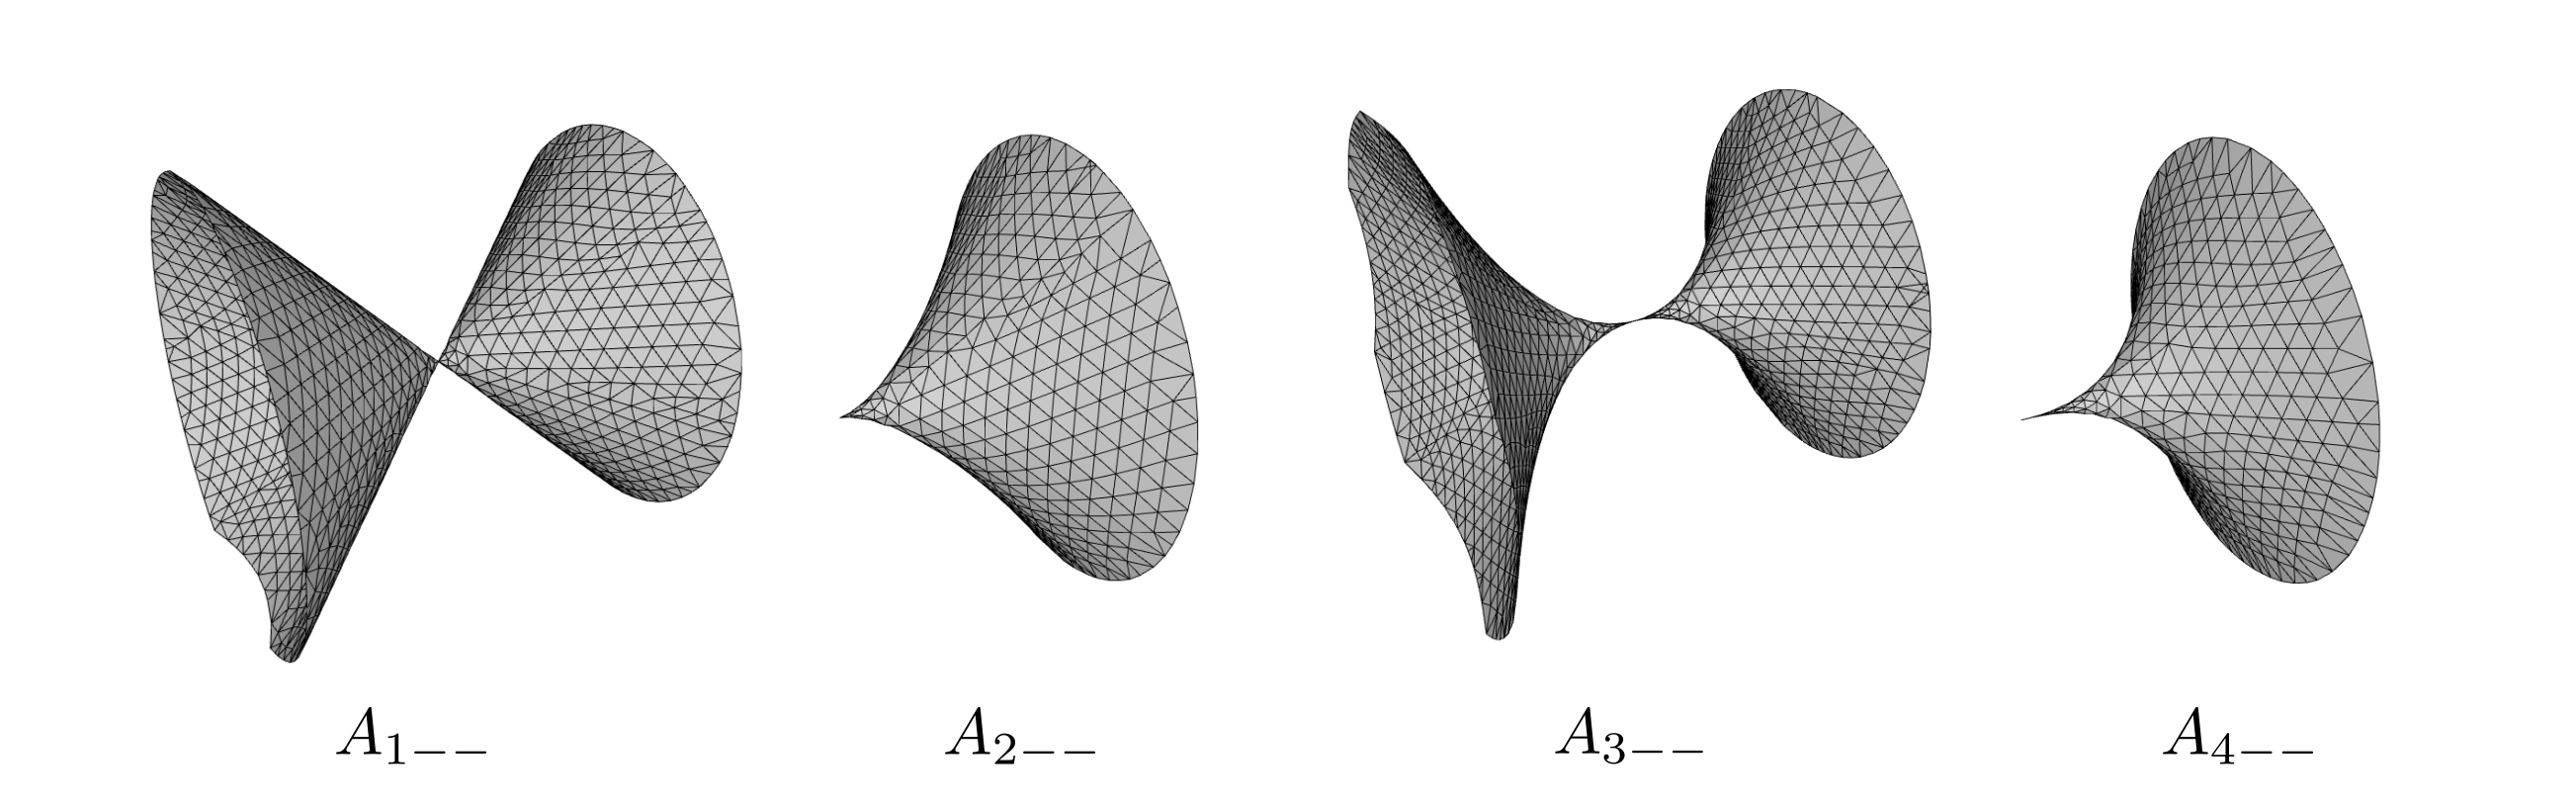
\includegraphics[scale=0.24]{images/img61}}
    \caption[Resulting uniform triangulation of $A_{n--}$ singularities]
    {Resulting uniform triangulation of $A_{n--}$ singularities with layers.}
    %id obrazku, pomocou ktoreho sa budeme na obrazok odvolavat
    \label{img:61}
\end{figure} 

The resulting adaptive meshes from our algorithm can be seen on the 
Figure~\ref{img:60}.
\begin{figure}[h!]
    \centerline{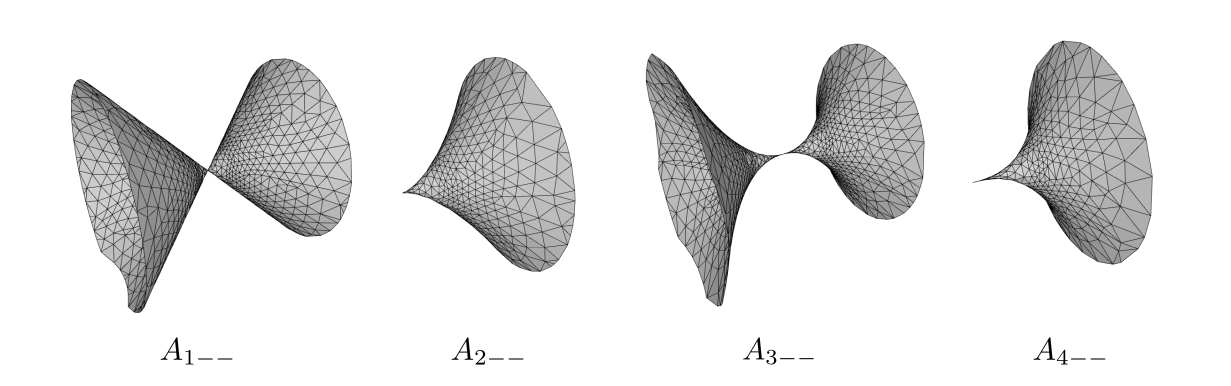
\includegraphics[scale=0.5]{images/img60}}
    \caption[Resulting adaptive triangulation of $A_{n--}$ singularities]
    {Resulting adaptive triangulation of $A_{n--}$ singularities with layers.}
    %id obrazku, pomocou ktoreho sa budeme na obrazok odvolavat
    \label{img:60}
\end{figure}

The resulting meshes generated by SingSurf 
can be seen on the Figure~\ref{img:47}.
\begin{figure}[h!]
    \centerline{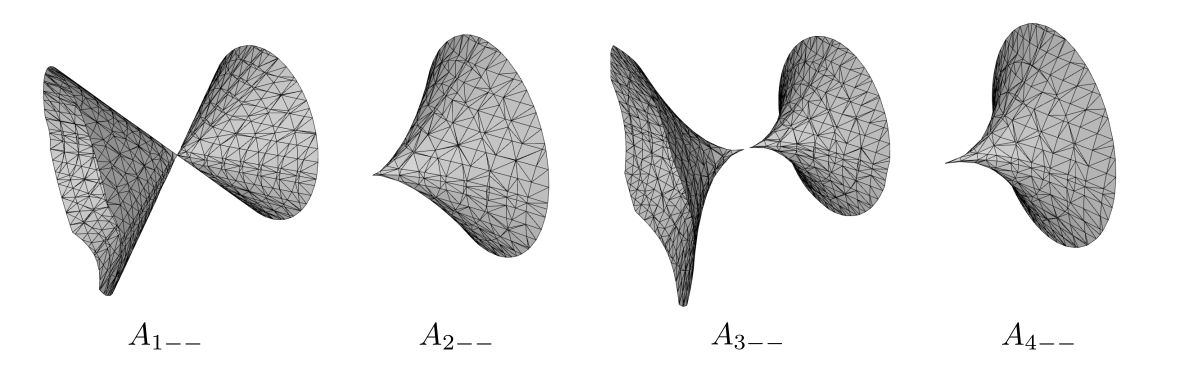
\includegraphics[scale=0.5]{images/img47}}
    \caption[Resulting triangulation of $A_{n--}$ singularities by SingSurf]
    {Resulting triangulation of $A_{n--}$ singularities by SingSurf \cite{morris2003client}.}
    %id obrazku, pomocou ktoreho sa budeme na obrazok odvolavat
    \label{img:47}
\end{figure}

The comparison on the quality criteria measured on these meshes 
is in the table~\ref{tab:An--}. The better values are visualized
by the green color and the worse values are visualized by the red 
color.
\renewcommand*{\MinNumberA}{0.0}%
\renewcommand*{\MaxNumberA}{1.0}%
\pgfmathsetmacro{\MidNumberA}{(\MinNumberA+\MaxNumberA)/2}%
\renewcommand*{\MinNumberB}{0.0}%
\renewcommand*{\MaxNumberB}{0.020}%
\pgfmathsetmacro{\MidNumberB}{(\MinNumberB+\MaxNumberB)/2}%
\renewcommand*{\MinNumberC}{0.0}%
\renewcommand*{\MaxNumberC}{0.01}%
\pgfmathsetmacro{\MidNumberC}{(\MinNumberC+\MaxNumberC)/2}%
\renewcommand*{\MinNumberD}{0.010}%
\renewcommand*{\MaxNumberD}{0.052}%
\pgfmathsetmacro{\MidNumberD}{(\MinNumberD+\MaxNumberD)/2}%


\begin{table}[h!]
    \caption[Quality criteria -- $A_{n--}$ singularities]{Comparison of the quality criteria for $A_{n--}$ singularities.}
        \begin{center}
        \label{tab:An--}
            \begin{tabular}{|c|c|A B C D|} 
                \hline
                \hline
                \multicolumn{6}{|c|}{$A_{n--}$ singularities} \\
                \hline
                \hline
                \hspace{3mm} type \hspace{3mm} & \hspace{20mm} \hspace{20mm} & $k_1$ & $k_2$ & $k_3$ & $k_4$ \EndTableHeader\\
                \hline
                \hline
                \multirow{3}{*}{$A_{1--}$} & SingSurf & 0.113 & 0.015 & 0.001 & 0.052\\
                \cline{2-6} 
                                            & Uniform algorithm & 0.834 & 0.007 & 0.001 & 0.010\\
                \cline{2-6} 
                                            & Adaptive algorithm & 0.760 & 0.011 & 0.002 & 0.017\\
                \hline
                \hline 
                \multirow{3}{*}{$A_{2--}$} & SingSurf & 0.077 & 0.008 & 0.001 & 0.051\\
                \cline{2-6}
                                            & Uniform algorithm & 0.793 & 0.008 & 0.001 & 0.010\\
                \cline{2-6} 
                                            & Adaptive algorithm & 0.729 & 0.008 & 0.001 & 0.017\\
                \hline
                \hline
                \multirow{3}{*}{$A_{3--}$} & SingSurf & 0.049 & 0.012 & 0.001 & 0.048\\
                \cline{2-6}
                                            & Uniform algorithm & 0.651 & 0.008 & 0.001 & 0.011\\
                \cline{2-6} 
                                            & Adaptive algorithm & 0.599 & 0.008 & 0.001 & 0.018\\
                \hline
                \hline
                \multirow{3}{*}{$A_{4--}$} & SingSurf & 0.325 & 0.020 & 0.001 & 0.045\\
                \cline{2-6}
                                            & Uniform algorithm & 0.309 & 0.008 & 0.001 & 0.014\\
                \cline{2-6} 
                                            & Adaptive algorithm & 0.365 & 0.008 & 0.001 & 0.020\\
                \hline
                \hline
            \end{tabular}
        \end{center}
    \end{table}

\clearpage
\subsubsection*{$A_{n+-}$ singularities}
We created meshes of $A_{2+-}, A_{3+-}$ and $A_{4+-}$ singularities.

The resulting uniform meshes from our algorithm can be seen on the 
Figure~\ref{img:63}.
\begin{figure}[h!]
    \centerline{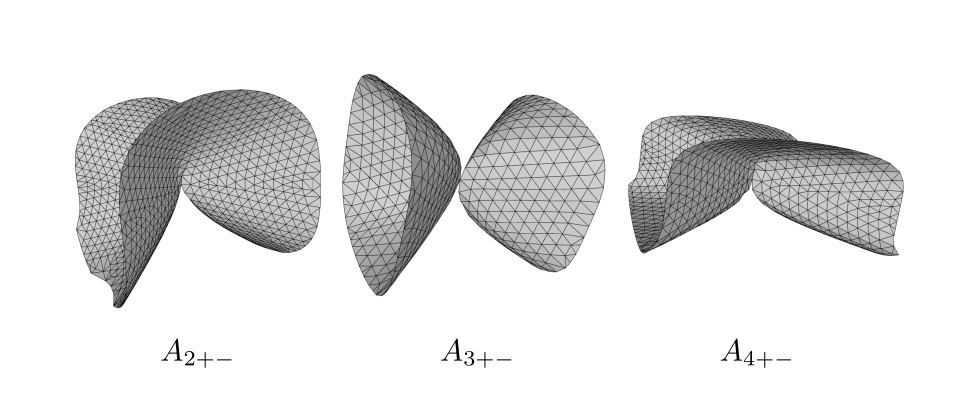
\includegraphics[scale=0.5]{images/img63}}
    \caption[Resulting uniform triangulation of $A_{n+-}$ singularities]
    {Resulting uniform triangulation of $A_{n+-}$ singularities with layers.}
    %id obrazku, pomocou ktoreho sa budeme na obrazok odvolavat
    \label{img:63}
\end{figure}

The resulting adaptive meshes from our algorithm can be seen on the 
Figure~\ref{img:65}.
\begin{figure}[h!]
    \centerline{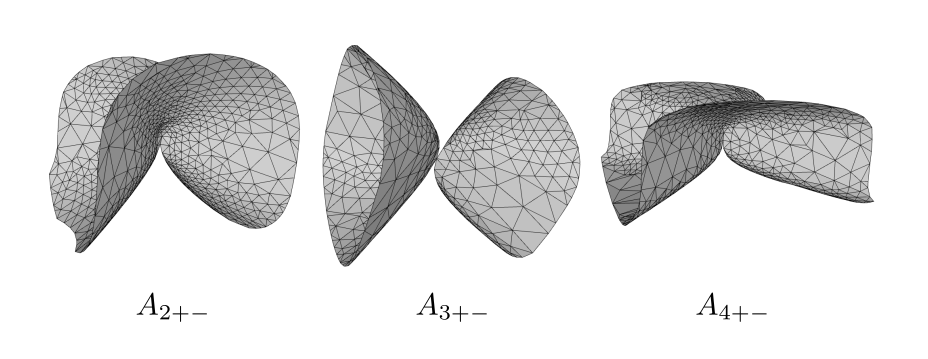
\includegraphics[scale=0.5]{images/img65}}
    \caption[Resulting adaptive triangulation of $A_{n+-}$ singularities]
    {Resulting adaptive triangulation of $A_{n+-}$ singularities with layers.}
    %id obrazku, pomocou ktoreho sa budeme na obrazok odvolavat
    \label{img:65}
\end{figure}

The resulting meshes generated by SingSurf 
can be seen on the Figure~\ref{img:47}.
\begin{figure}[h!]
    \centerline{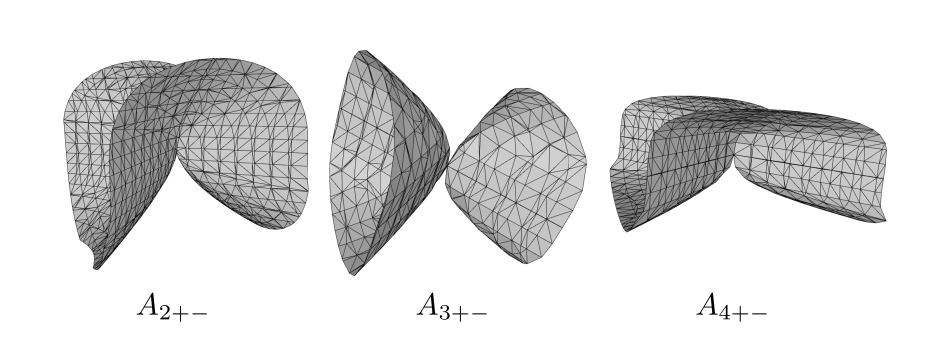
\includegraphics[scale=0.5]{images/img68}}
    \caption[Resulting triangulation of $A_{n+-}$ singularities by SingSurf]
    {Resulting triangulation of $A_{n+-}$ singularities by SingSurf \cite{morris2003client}.}
    %id obrazku, pomocou ktoreho sa budeme na obrazok odvolavat
    \label{img:68}
\end{figure}
The comparison on the quality criteria measured on these meshes 
is in the table~\ref{tab:An+-}. The better values are visualized
by the green color and the worse values are visualized by the red 
color.

\renewcommand*{\MinNumberA}{0.0}%
\renewcommand*{\MaxNumberA}{1.0}%
\pgfmathsetmacro{\MidNumberA}{(\MinNumberA+\MaxNumberA)/2}%
\renewcommand*{\MinNumberB}{0.008}%
\renewcommand*{\MaxNumberB}{0.061}%
\pgfmathsetmacro{\MidNumberB}{(\MinNumberB+\MaxNumberB)/2}%
\renewcommand*{\MinNumberC}{0.00}%
\renewcommand*{\MaxNumberC}{0.01}%
\pgfmathsetmacro{\MidNumberC}{(\MinNumberC+\MaxNumberC)/2}% 
\renewcommand*{\MinNumberD}{0.011}%
\renewcommand*{\MaxNumberD}{0.118}%
\pgfmathsetmacro{\MidNumberD}{(\MinNumberD+\MaxNumberD)/2}%


\begin{table}[h!]
    \caption[Quality criteria -- $A_{n+-}$ singularities]{Comparison of the quality criteria for $A_{n+-}$ singularities.}
        \begin{center}
        \label{tab:An+-}
            \begin{tabular}{|c|c|A B C D|} 
                \hline
                \hline
                \multicolumn{6}{|c|}{$A_{n+-}$ singularities} \\
                \hline
                \hline
                \hspace{3mm} type \hspace{3mm} & \hspace{20mm} \hspace{20mm} & $k_1$ & $k_2$ & $k_3$ & $k_4$ \EndTableHeader\\
                \hline
                \hline
                \multirow{3}{*}{$A_{2+-}$} & SingSurf       & 0.189 & 0.017 & 0.002 & 0.052\\
                \cline{2-6}
                                            & Uniform algorithm & 0.839 & 0.017 & 0.001 & 0.010\\
                \cline{2-6} 
                                            & Adaptive algorithm & 0.739 & 0.008 & 0.001 & 0.019\\
                \hline
                \hline
                \multirow{3}{*}{$A_{3+-}$} & SingSurf       & 0.001 & 0.042 & 0.005 & 0.073\\
                \cline{2-6}
                                            & Uniform algorithm & 0.868 & 0.019 & 0.003 & 0.014\\
                \cline{2-6} 
                                            & Adaptive algorithm & 0.732 & 0.017 & 0.003 & 0.029\\
                \hline
                \hline
                \multirow{3}{*}{$A_{4+-}$} & SingSurf       & 0.001 & 0.061 & 0.006 & 0.118\\
                \cline{2-6}
                                            & Uniform algorithm & 0.839 & 0.053 & 0.006 & 0.030\\
                \cline{2-6} 
                                            & Adaptive algorithm & 0.711 & 0.032 & 0.006 & 0.063\\
                \hline
                \hline 
            \end{tabular}
        \end{center} 
    \end{table}
    

    \clearpage

    \subsubsection*{$D_{n}$ singularities}
    We created meshes of $D_{4+-}, D_{4--}, D_{5+-}$ and $D_{5--}$ singularities.

    The resulting uniform meshes from our algorithm can be seen on the 
    Figure~\ref{img:62}.
    \begin{figure}[h!]
        \centerline{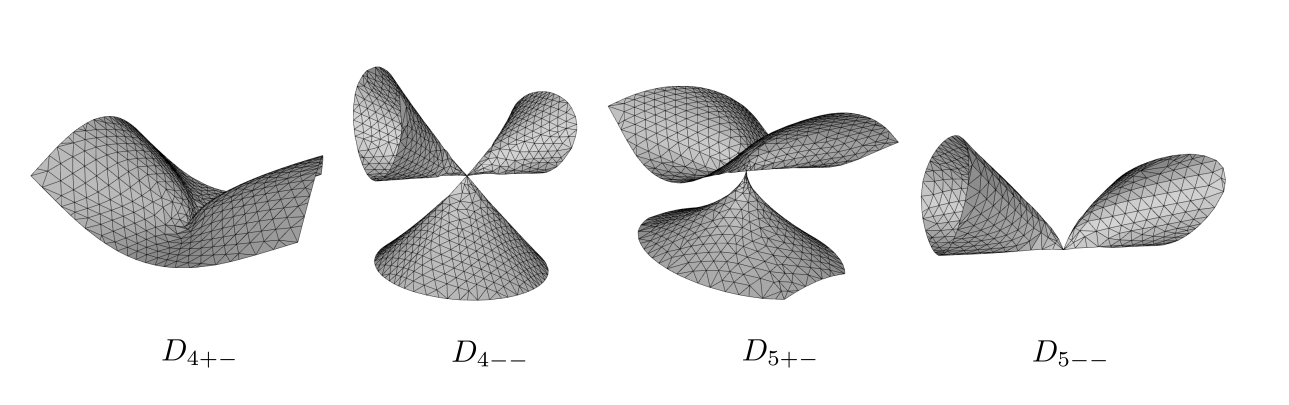
\includegraphics[scale=0.5]{images/img62}}
        \caption[Resulting uniform triangulation of $D_{n}$ singularities]
        {Resulting uniform triangulation of $D_{n}$ singularities with layers.}
        %id obrazku, pomocou ktoreho sa budeme na obrazok odvolavat
        \label{img:62}
    \end{figure}

    The resulting adaptive meshes from our algorithm can be seen on the 
    Figure~\ref{img:66}.
    \begin{figure}[h!]
        \centerline{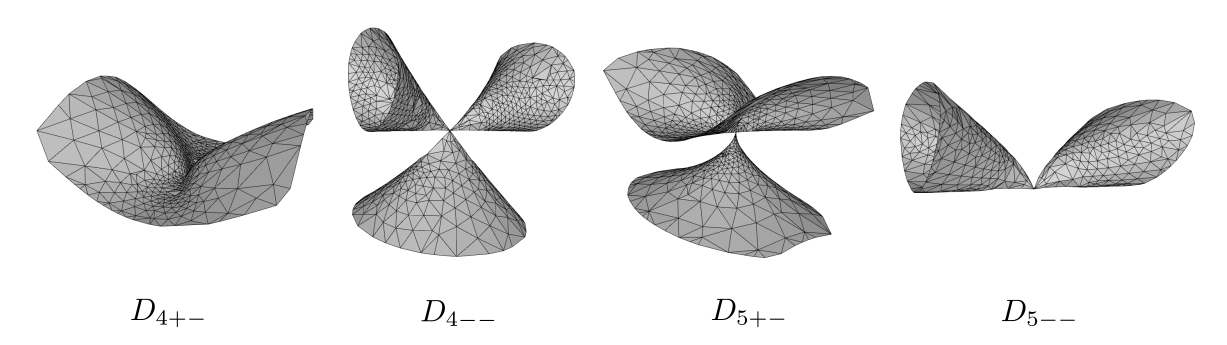
\includegraphics[scale=0.5]{images/img66}}
        \caption[Resulting adaptive triangulation of $D_{n}$ singularities]
        {Resulting adaptive triangulation of $A_{n}$ singularities with layers.}
        %id obrazku, pomocou ktoreho sa budeme na obrazok odvolavat
        \label{img:66}
    \end{figure}

    The resulting meshes generated by SingSurf 
    can be seen on the Figure~\ref{img:69}.
    \begin{figure}[h!]
        \centerline{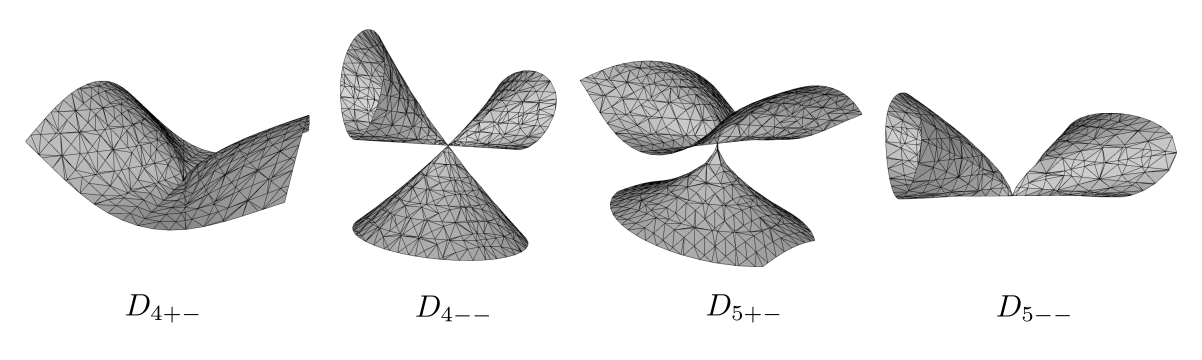
\includegraphics[scale=0.5]{images/img69}}
        \caption[Resulting triangulation of $D_{n}$ singularities by SingSurf]
        {Resulting triangulation of $D_{n}$ singularities by SingSurf \cite{morris2003client}.}
        %id obrazku, pomocou ktoreho sa budeme na obrazok odvolavat
        \label{img:69}
    \end{figure}
    The comparison on the quality criteria measured on these meshes 
    is in the table~\ref{tab:Dn}. The better values are visualized
    by the green color and the worse values are visualized by the red 
    color.

\renewcommand*{\MinNumberA}{0.0}%
\renewcommand*{\MaxNumberA}{1.0}% 
\pgfmathsetmacro{\MidNumberA}{(\MinNumberA+\MaxNumberA)/2}%
\renewcommand*{\MinNumberB}{0.017}%
\renewcommand*{\MaxNumberB}{0.032}%
\pgfmathsetmacro{\MidNumberB}{(\MinNumberB+\MaxNumberB)/2}%
\renewcommand*{\MinNumberC}{0.0}%
\renewcommand*{\MaxNumberC}{0.01}%
\pgfmathsetmacro{\MidNumberC}{(\MinNumberC+\MaxNumberC)/2}% 
\renewcommand*{\MinNumberD}{0.013}%
\renewcommand*{\MaxNumberD}{0.078}%
\pgfmathsetmacro{\MidNumberD}{(\MinNumberD+\MaxNumberD)/2}%


\begin{table}[h!]
    \caption[Quality criteria -- $D_{n}$ singularities]{Comparison of the quality criteria for $D_{n}$ singularities.}
        \begin{center}
        \label{tab:Dn}
        \begin{tabular}{|c|c|A B C D|} 
            \hline
            \hline
            \multicolumn{6}{|c|}{$D_{n}$ singularities} \\
            \hline
            \hline
            \hspace{3mm} type \hspace{3mm} & \hspace{20mm} \hspace{20mm} & $k_1$ & $k_2$ & $k_3$ & $k_4$ \EndTableHeader\\
            \hline
            \hline
            \multirow{3}{*}{$D_{4--}$} & SingSurf       & 0.091 & 0.017 & 0.002 & 0.052\\
            \cline{2-6}
                                        & Uniform algorithm & 0.761 & 0.023 & 0.002 & 0.013\\
            \cline{2-6} 
                                        & Adaptive algorithm & 0.686 & 0.025 & 0.002 & 0.020\\
            \hline
            \hline
            \multirow{3}{*}{$D_{4+-}$} & SingSurf       & 0.094 & 0.028 & 0.003 & 0.078\\
            \cline{2-6}
                                        & Uniform algorithm & 0.650 & 0.032 & 0.003 & 0.027\\
            \cline{2-6} 
                                        & Adaptive algorithm & 0.713 & 0.028 & 0.003 & 0.040\\
            \hline
            \hline
            \multirow{3}{*}{$D_{5--}$} & SingSurf       & 0.001 & 0.032 & 0.006 & 0.076\\
            \cline{2-6}
                                        & Uniform algorithm & 0.763 & 0.059 & 0.005 & 0.026\\
            \cline{2-6} 
                                        & Adaptive algorithm & 0.685 & 0.061 & 0.006 & 0.040\\
            \hline
            \hline 
            \multirow{3}{*}{$D_{5+-}$} & SingSurf       & 0.132 & 0.029 & 0.003 & 0.076\\
            \cline{2-6}
                                        & Uniform algorithm & 0.747 & 0.030 & 0.003 & 0.027\\
            \cline{2-6} 
                                        & Adaptive algorithm & 0.670 & 0.027 & 0.003 & 0.038\\
            \hline
            \hline 
        \end{tabular}
    \end{center} 
\end{table}

    
\renewcommand*{\MinNumberA}{0.0}%
\renewcommand*{\MaxNumberA}{1.0}%
\pgfmathsetmacro{\MidNumberA}{(\MinNumberA+\MaxNumberA)/2}%
\renewcommand*{\MinNumberB}{0.013}%
\renewcommand*{\MaxNumberB}{0.045}%
\pgfmathsetmacro{\MidNumberB}{(\MinNumberB+\MaxNumberB)/2}%
\renewcommand*{\MinNumberC}{0.0}%
\renewcommand*{\MaxNumberC}{0.01}%
\pgfmathsetmacro{\MidNumberC}{(\MinNumberC+\MaxNumberC)/2}% 
\renewcommand*{\MinNumberD}{0.017}%
\renewcommand*{\MaxNumberD}{0.110}%
\pgfmathsetmacro{\MidNumberD}{(\MinNumberD+\MaxNumberD)/2}%

\clearpage
\subsubsection*{$E_{n}$ singularities}
    We created meshes of $E_{4++}, E_{6+-}, E_{7++}$ and $E_{8++}$ singularities.

    The resulting uniform meshes from our algorithm can be seen on the 
    Figure~\ref{img:64}.
    \begin{figure}[h!]
        \centerline{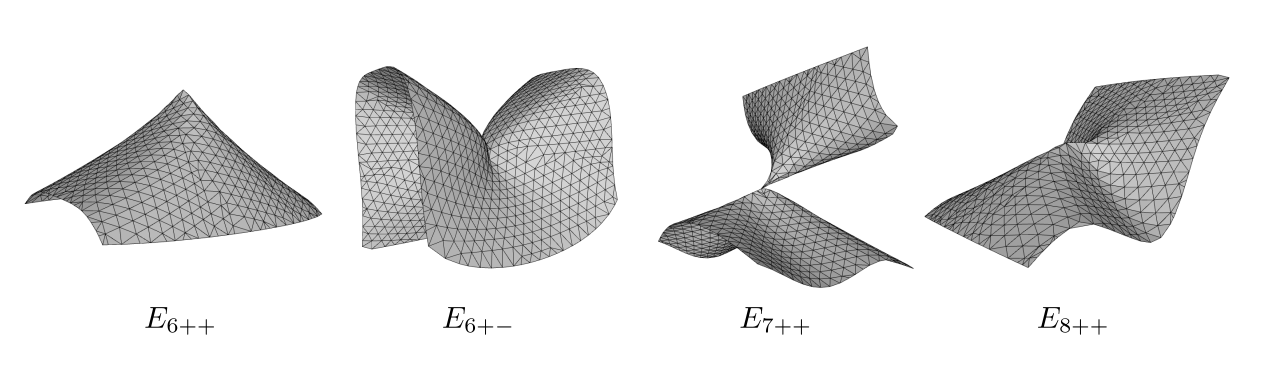
\includegraphics[scale=0.5]{images/img64}}
        \caption[Resulting uniform triangulation of $E_{n}$ singularities]
        {Resulting uniform triangulation of $E_{n}$ singularities with layers.}
        %id obrazku, pomocou ktoreho sa budeme na obrazok odvolavat
        \label{img:64}
    \end{figure}

    The resulting adaptive meshes from our algorithm can be seen on the 
    Figure~\ref{img:67}.
    \begin{figure}[h!]
        \centerline{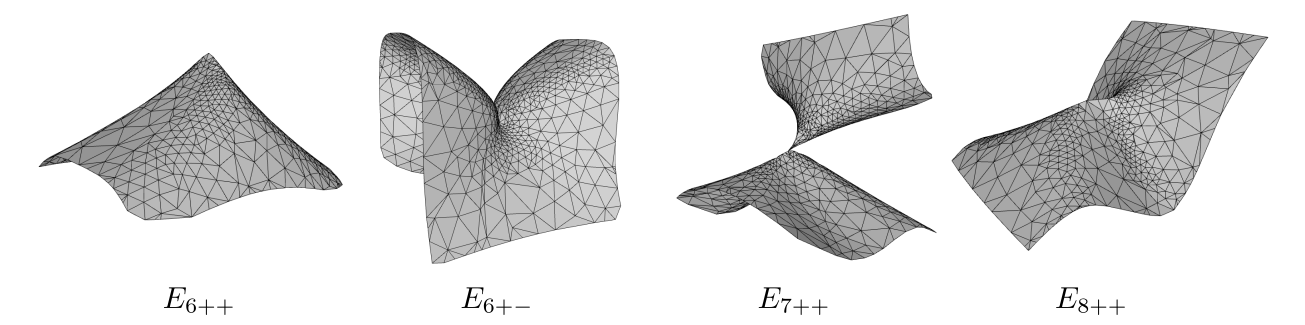
\includegraphics[scale=0.5]{images/img67}}
        \caption[Resulting adaptive triangulation of $E_{n}$ singularities]
        {Resulting adaptive triangulation of $E_{n}$ singularities with layers.}
        %id obrazku, pomocou ktoreho sa budeme na obrazok odvolavat
        \label{img:67}
    \end{figure}

    The resulting meshes generated by SingSurf 
can be seen on the Figure~\ref{img:70}.
\begin{figure}[h!]
    \centerline{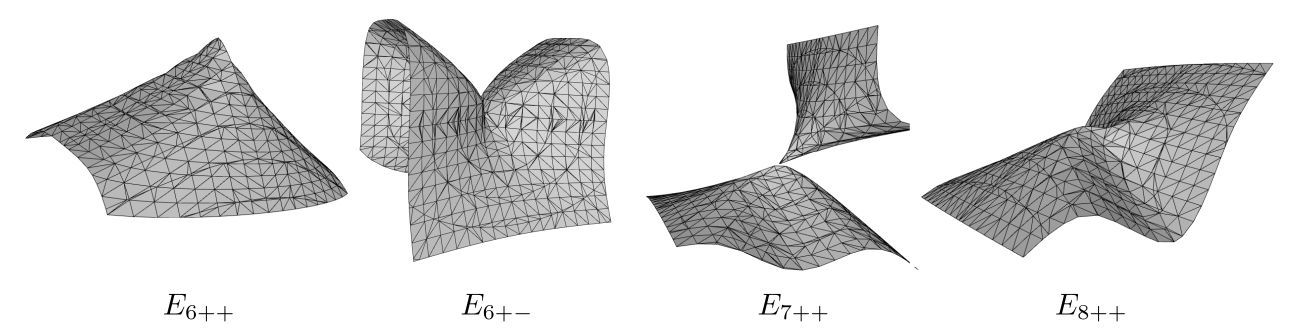
\includegraphics[scale=0.5]{images/img70}}
    \caption[Resulting triangulation of $E_{n}$ singularities by SingSurf]
    {Resulting triangulation of $E_{n}$ singularities by SingSurf \cite{morris2003client}.}
    %id obrazku, pomocou ktoreho sa budeme na obrazok odvolavat
    \label{img:70}
\end{figure}

The comparison on the quality criteria measured on these meshes 
is in the table~\ref{tab:En}. The better values are visualized
by the green color and the worse values are visualized by the red 
color.

\begin{table}[h!]
    \caption[Quality criteria -- $E_{n}$ singularities]{Comparison of the quality criteria for $E_{n}$ singularities.}
        \begin{center}
        \label{tab:En}
        \begin{tabular}{|c|c|A B C D|}
            \hline
            \hline
            \multicolumn{6}{|c|}{$E_{n}$ singularities} \\
            \hline
            \hline
            \hspace{3mm} type \hspace{3mm} & \hspace{20mm} \hspace{20mm} & $k_1$ & $k_2$ & $k_3$ & $k_4$ \EndTableHeader\\
            \hline
            \hline
            \multirow{3}{*}{$E_{6++}$} & SingSurf       & 0.006 & 0.043 & 0.003 & 0.069\\
            \cline{2-6}
                                        & Uniform algorithm & 0.831 & 0.013 & 0.002 & 0.017\\
            \cline{2-6} 
                                        & Adaptive algorithm & 0.738 & 0.021 & 0.002 & 0.030\\
            \hline
            \hline
            \multirow{3}{*}{$E_{6+-}$} & SingSurf       & 0.011 & 0.040 & 0.003 & 0.077\\
            \cline{2-6}
                                        & Uniform algorithm & 0.842 & 0.014 & 0.002 & 0.017\\
            \cline{2-6} 
                                        & Adaptive algorithm & 0.721 & 0.034 & 0.002 & 0.034\\
            \hline
            \hline
            \multirow{3}{*}{$E_{7++}$} & SingSurf       & 0.198 & 0.024 & 0.004 & 0.110\\
            \cline{2-6}
                                        & Uniform algorithm & 0.797 & 0.027 & 0.004 & 0.027\\
            \cline{2-6} 
                                        & Adaptive algorithm & 0.673 & 0.028 & 0.004 & 0.048\\
            \hline
            \hline 
            \multirow{3}{*}{$E_{8++}$} & SingSurf       & 0.260 & 0.045 & 0.004 & 0.100\\
            \cline{2-6}
                                        & Uniform algorithm & 0.803 & 0.028 & 0.004 & 0.032\\
            \cline{2-6} 
                                        & Adaptive algorithm & 0.703 & 0.022 & 0.004 & 0.056\\
            \hline 
            \hline 
        \end{tabular}
    \end{center} 
\end{table}

\section{Curve singularities}
In this section we will present the meshes generated for the intersection, union 
and difference of the interiors of two regular surfaces.
The uniform meshes are generated with multiple different edges length.

\subsection{Intersection}
The intersection of the inside of a sphere given by the equation
$x^2+y^2+z^2-4=0$ and the inside of a hyperboloid given by the 
equation $x^2-y^2+z^2-1=0$ is displayed on the Figure~\ref{img:71}.
\begin{figure}[h!]
    \centerline{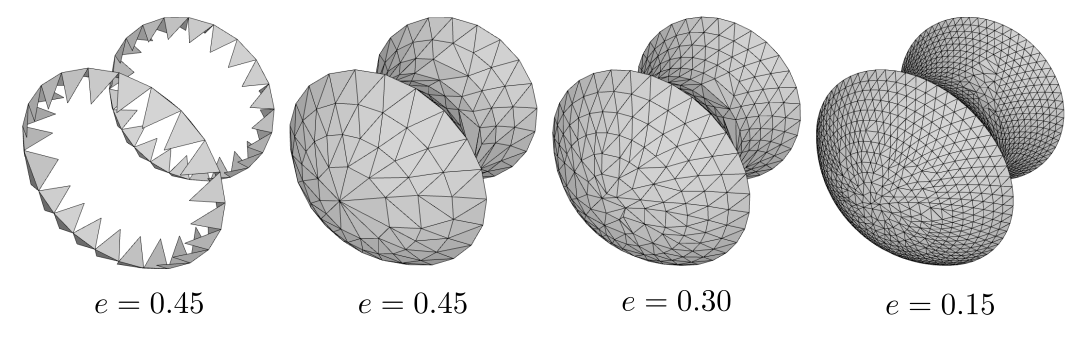
\includegraphics[scale=0.5]{images/img71}}
    \caption[The surface given by the intersection of a sphere and a hyperboloid]
    {The surface given by the intersection of a sphere and a hyperboloid.}
    %id obrazku, pomocou ktoreho sa budeme na obrazok odvolavat
    \label{img:71}
\end{figure}

The intersection of the inside of a sphere given by the equation
$x^2+y^2+z^2-9=0$ and the inside of a tanglecube given by the 
equation $x^4-5x^2+y^4-5y^2+z^4-5z^2+11.8=0$ is displayed on the Figure~\ref{img:73}.
\begin{figure}[h!]
    \centerline{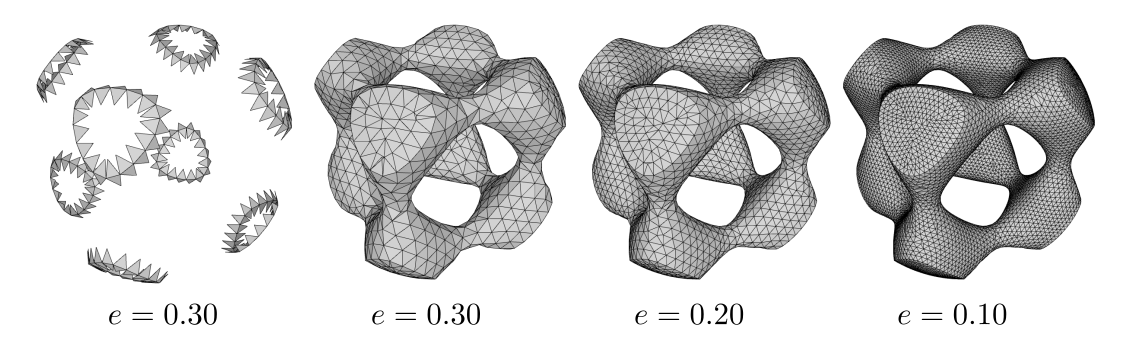
\includegraphics[scale=0.5]{images/img73}}
    \caption[The surface given by the intersection of a sphere and a tanglecube]
    {The surface given by the intersection of a sphere and a tanglecube.}
    %id obrazku, pomocou ktoreho sa budeme na obrazok odvolavat
    \label{img:73}
\end{figure}

The intersection of the inside of a blobby object given by the equation
\newline
$2\sqrt{x^2+y^2+z^2+1}-1.1=0$ 
and the inside of a plane (halfspace) given by the 
equation $z=0$ is displayed on the Figure~\ref{img:74}.
\begin{figure}[h!]
    \centerline{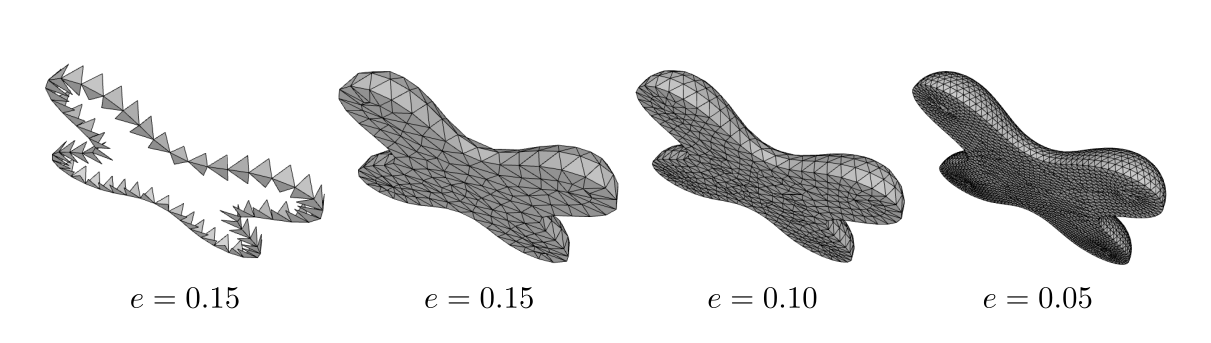
\includegraphics[scale=0.5]{images/img74}}
    \caption[The surface given by the intersection of a blobby object and a plane]
    {The surface given by the intersection of a blobby object and a plane.}
    %id obrazku, pomocou ktoreho sa budeme na obrazok odvolavat
    \label{img:74}
\end{figure}

The intersection of the inside of a sphere given by the equation
$x^2+y^2+z^2-4=0$ and the inside of a plane (halfspace) given by the 
equation $y=$ is displayed on the Figure~\ref{img:72}.
\begin{figure}[h!]
    \centerline{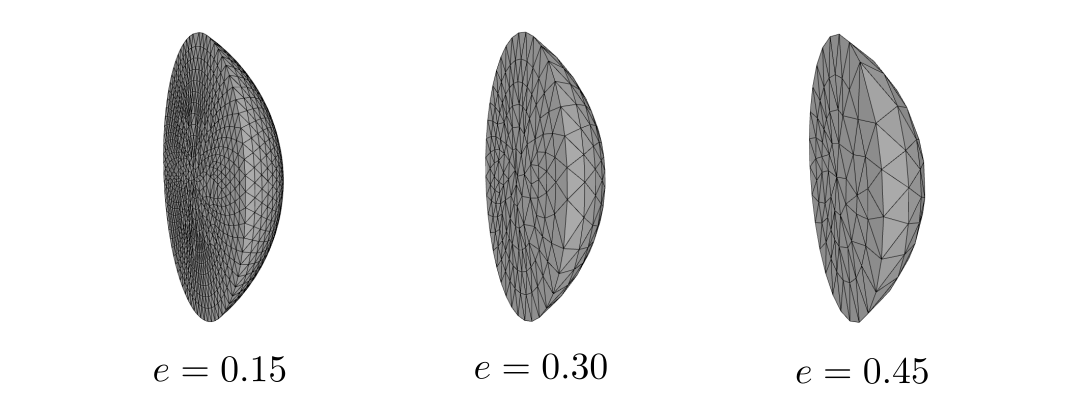
\includegraphics[scale=0.5]{images/img72}}
    \caption[The surface given by the intersection of a sphere and a plane]
    {The surface given by the intersection of a sphere and a plane.}
    %id obrazku, pomocou ktoreho sa budeme na obrazok odvolavat
    \label{img:72}
\end{figure}

\subsection{Union}
The union of the inside of a sphere given by the equation
$x^2+y^2+z^2-4=0$ and the inside of a hyperboloid given by the 
equation $x^2-y^2+z^2-1=0$ is displayed on the Figure~\ref{img:77}.
\begin{figure}[h!]
    \centerline{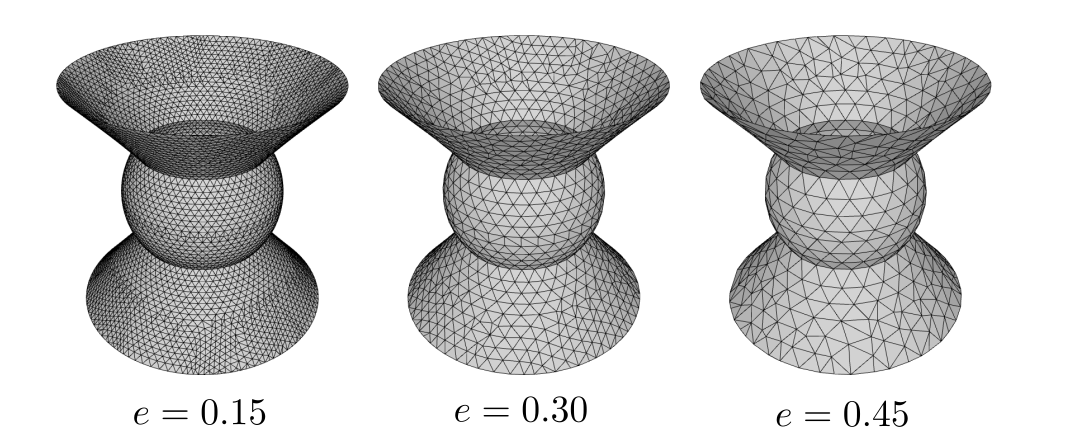
\includegraphics[scale=0.5]{images/img77}}
    \caption[The surface given by the union of a sphere and a hyperboloid]
    {The surface given by the union of a sphere and a hyperboloid.}
    %id obrazku, pomocou ktoreho sa budeme na obrazok odvolavat
    \label{img:77}
\end{figure}
The union of the inside of a sphere given by the equation
$x^2+y^2+z^2-4=0$ and the inside of a sphere given by the 
equation $(x-2)^2+y^2+z^2-4=0$ is displayed on the Figure~\ref{img:78}.
\begin{figure}[h!]
    \centerline{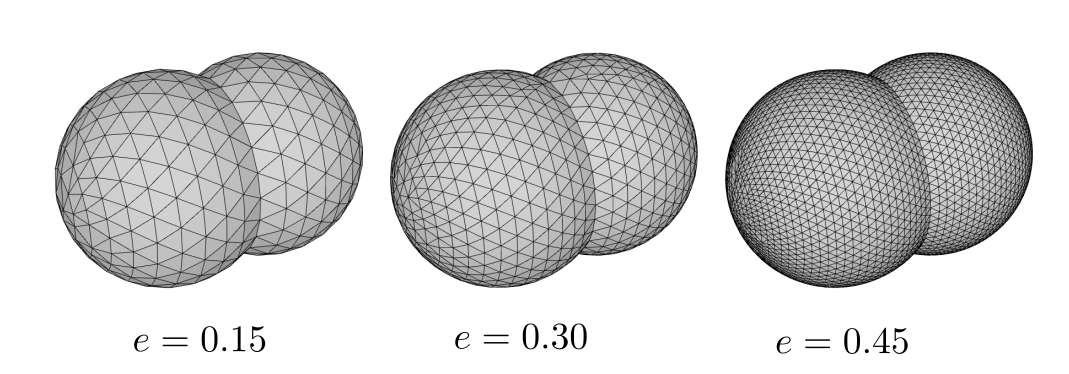
\includegraphics[scale=0.5]{images/img78}}
    \caption[The surface given by the union of two spheres]
    {The surface given by the union of two spheres.}
    %id obrazku, pomocou ktoreho sa budeme na obrazok odvolavat
    \label{img:78}
\end{figure}
The union of the inside of a sphere given by the equation
$x^2+y^2+z^2-9=0$ and the inside of a tanglecube given by the 
equation $x^4-5x^2+y^4-5y^2+z^4-5z^2+11.8=0$ is displayed on the Figure~\ref{img:79}.
\begin{figure}[h!]
    \centerline{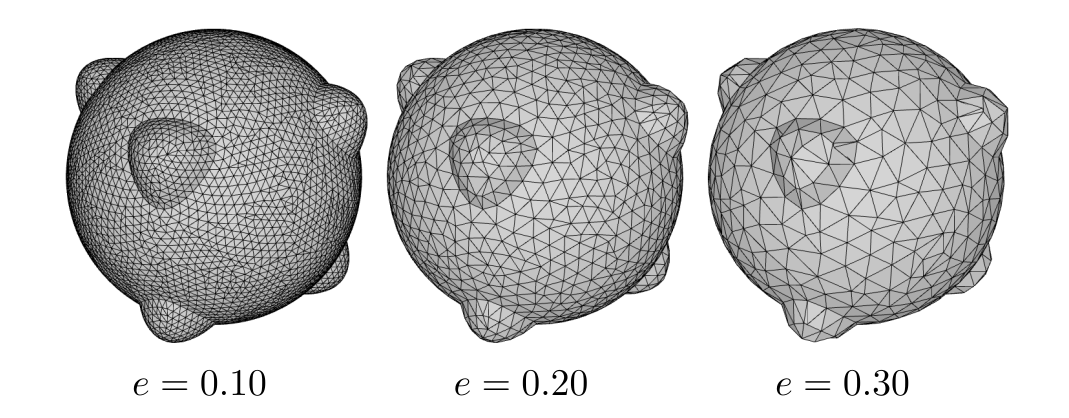
\includegraphics[scale=0.5]{images/img79}}
    \caption[The surface given by the union of a sphere and a tanglecube]
    {The surface given by the union of a sphere and a tanglecube.}
    %id obrazku, pomocou ktoreho sa budeme na obrazok odvolavat
    \label{img:79}
\end{figure}

\subsection{Difference}

The difference of the inside of a sphere given by the equation
$x^2+y^2+z^2-4=0$ and the inside of a sphere given by the 
equation $(x-2)^2+y^2+z^2-4=0$ is displayed on the Figure~\ref{img:80}.
\begin{figure}[h!]
    \centerline{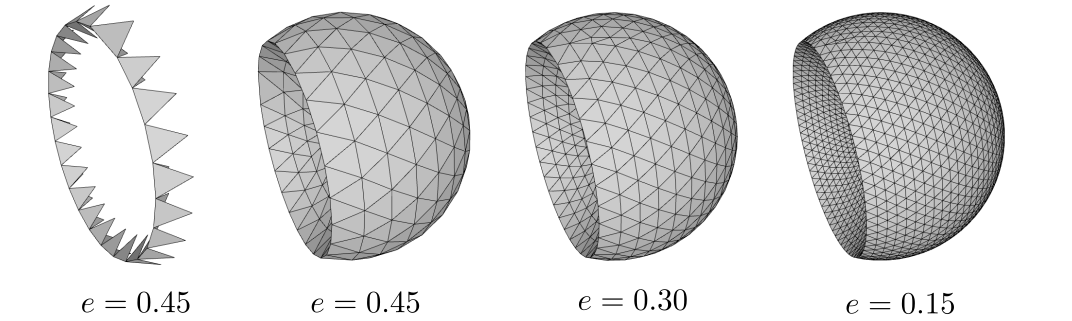
\includegraphics[scale=0.49]{images/img80}}
    \caption[The surface given by the difference of two spheres]
    {The surface given by the difference of two spheres.}
    %id obrazku, pomocou ktoreho sa budeme na obrazok odvolavat
    \label{img:80}
\end{figure}

The difference of the inside of a sphere given by the equation
$x^2+y^2+z^2-5.5=0$ and the inside of a tanglecube given by the 
equation $x^4-5x^2+y^4-5y^2+z^4-5z^2+11.8=0$ is displayed on the Figure~\ref{img:82}.
\begin{figure}[h!]
    \centerline{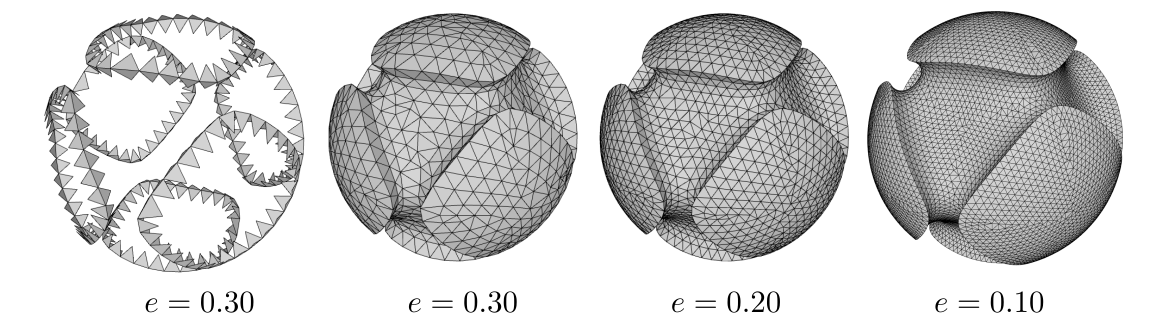
\includegraphics[scale=0.49]{images/img82}}
    \caption[The surface given by the difference of a sphere and a tanglecube]
    {The surface given by the difference of a sphere and a tanglecube.}
    %id obrazku, pomocou ktoreho sa budeme na obrazok odvolavat
    \label{img:82}
\end{figure}

The difference of the inside of a tanglecube given by the 
equation $x^4-5x^2+y^4-5y^2+z^4-5z^2+11.8=0$ and the inside 
of a sphere given by the equation
$x^2+y^2+z^2-5.5=0$ is displayed on the Figure~\ref{img:83}.
\begin{figure}[h!]
    \centerline{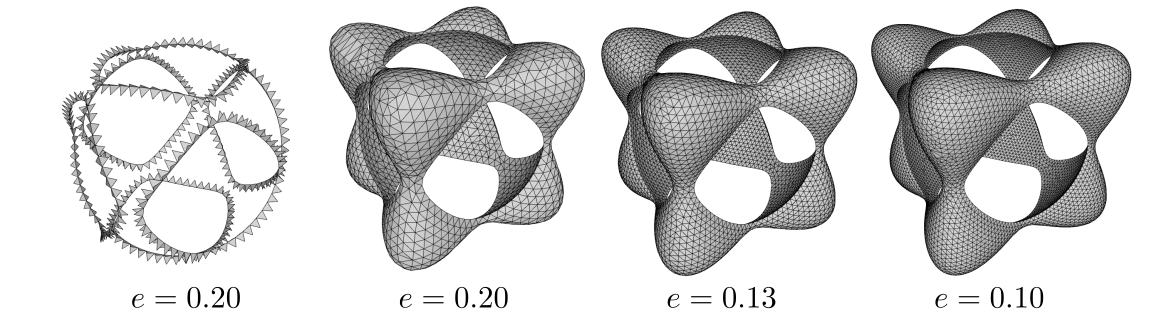
\includegraphics[scale=0.49]{images/img83}}
    \caption[The surface given by the difference of a tanglecube and a sphere]
    {The surface given by the difference of a tanglecube and a sphere.}
    %id obrazku, pomocou ktoreho sa budeme na obrazok odvolavat
    \label{img:83}
\end{figure}

\clearpage
\section{Results of the triangulation of a plane with multiple $A_{n--}$ singularities}
In this section we will present the meshes generated for the $A_{n--}$ singularities
sticked to the plane. The presented meshes are uniform with different edge lengths.

\textit{Note: Some edges of the mesh are not displayed due to zero angle between the incident
triangles. This is an error in the used obj viewer.}

The uniform mesh with a single $A_{2--}$ singularity sticked to a plane is displayed
on the Figure~\ref{img:84}.

\begin{figure}[h!]
    \centerline{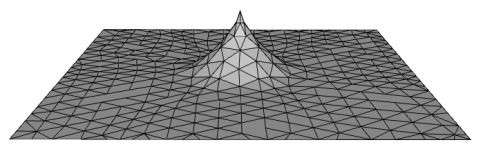
\includegraphics[scale=0.5]{images/img84}}
    \caption[The triangulation of the $A_{2--}$ singularity sticked to a plane]
    {The triangulation of the $A_{2--}$ singularity sticked to a plane.}
    %id obrazku, pomocou ktoreho sa budeme na obrazok odvolavat
    \label{img:84}
\end{figure}

The uniform mesh with a two $A_{2--}$ singularities sticked to a plane is displayed
on the Figure~\ref{img:85}.

\begin{figure}[h!]
    \centerline{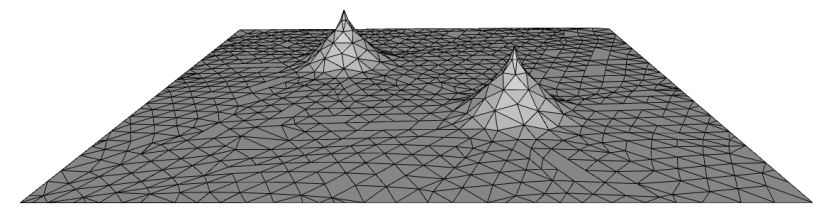
\includegraphics[scale=0.5]{images/img85}}
    \caption[The triangulation of the two $A_{2--}$ singularities sticked to a plane]
    {The triangulation of the two $A_{2--}$ singularities sticked to a plane.}
    %id obrazku, pomocou ktoreho sa budeme na obrazok odvolavat
    \label{img:85}
\end{figure}

The uniform mesh with one $A_{2--}$ singularity and one $A_{4--}$ singularity
sticked to a plane is displayed on the Figure~\ref{img:86}.

\begin{figure}[h!]
    \centerline{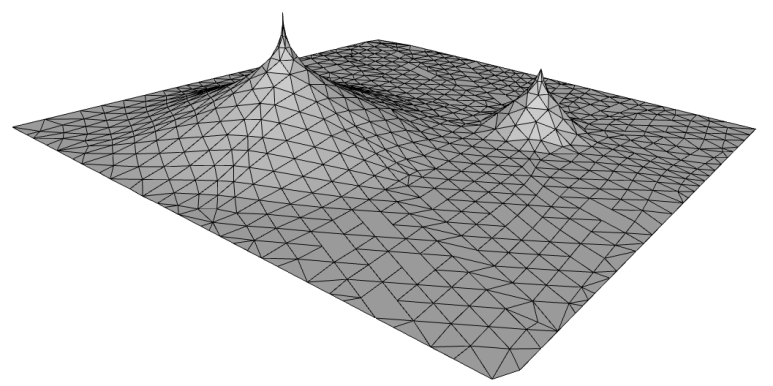
\includegraphics[scale=0.5]{images/img86}}
    \caption[The triangulation of $A_{2--}$ and $A_{4--}$ singularities sticked to a plane]
    {The triangulation of  $A_{2--}$ and $A_{4--}$ singularities sticked to a plane.}
    %id obrazku, pomocou ktoreho sa budeme na obrazok odvolavat
    \label{img:86}
\end{figure}

The uniform mesh with $A_{1--}$, $A_{2--}$, $A_{3--}$, $A_{4--}$ singularities
sticked to a plane is displayed on the Figure~\ref{img:87}.

\begin{figure}[h!]
    \centerline{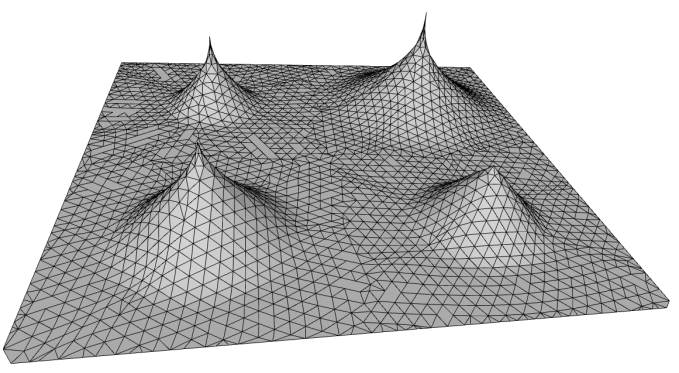
\includegraphics[scale=0.5]{images/img87}}
    \caption[The triangulation of $A_{1--}$, $A_{2--}$, $A_{3--}$ and $A_{4--}$ singularities sticked to a plane]
    {The triangulation of $A_{1--}$, $A_{2--}$, $A_{3--}$ and $A_{4--}$ singularities sticked to a plane.}
    %id obrazku, pomocou ktoreho sa budeme na obrazok odvolavat
    \label{img:87}
\end{figure}

\section{Computational speed comparison of the reimplemented solution}
\label{sub4.3}
In this section we compare the runtime of the reimplemented solution using half-edge 
and range-tree to the brute-force solution implemented in \cite{korecova2021triangulation}.

To obtain the results, laptop with 6-core AMD Ryzen 5 5600U with Radeon Graphics is used.

Plotting from data:

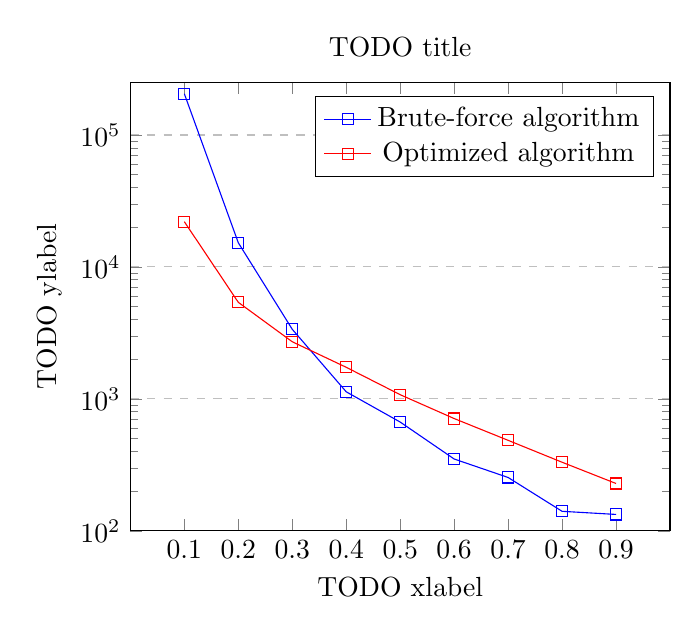
\begin{tikzpicture}
\begin{semilogyaxis}[
    title={TODO title},
    xlabel={TODO xlabel},
    ylabel={TODO ylabel},
    xmin=0, xmax=1,
    ymin=100, ymax=250000,
    xtick={0.1,0.2,0.3,0.4,0.5,0.6,0.7,0.8,0.9},
    ytick={100, 1000, 10000, 100000},
    legend pos=north east,
    ymajorgrids=true,
    grid style=dashed,
]

\addplot[
    color=blue,
    mark=square,
    ]
    coordinates {
    (0.1,205438.933)(0.2,15250.317)(0.3,3367.879)(0.4,1131.365)(0.5,667.250)(0.6,350.175)(0.7,253.612)(0.8,140.533)(0.9,133.069)
    };
    
\addplot[
    color=red,
    mark=square,
    ]
    coordinates {
    (0.1,22024.978)(0.2,5393.445)(0.3,2709.244)(0.4,1735.185)(0.5,1075.388)(0.6,709.317)(0.7,484.937)(0.8,330.943)(0.9,228.294)
    };
\legend{Brute-force algorithm, Optimized algorithm}
\end{semilogyaxis}
\end{tikzpicture}

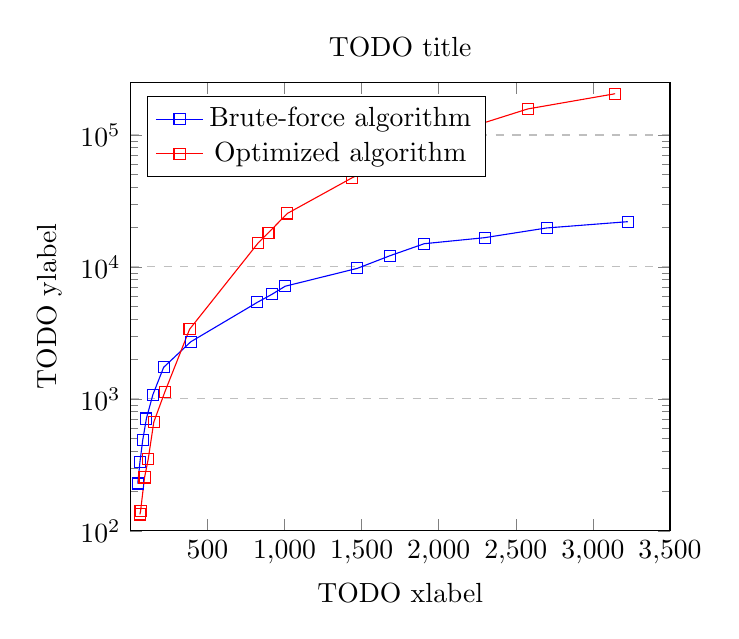
\begin{tikzpicture}
    \begin{semilogyaxis}[
        title={TODO title},
        xlabel={TODO xlabel},
        ylabel={TODO ylabel},
        xmin=0, xmax=3500,
        ymin=100, ymax=250000,
        xtick={500,1000,1500,2000,2500,3000,3500},
        ytick={100, 1000, 10000, 100000},
        legend pos=north west,
        ymajorgrids=true,
        grid style=dashed,
    ]
    
    \addplot[
        color=blue,
        mark=square,
        ]
        coordinates {
        (48,228.294)(62,330.943)(80,484.937)(104,709.317)
        (146,1075.388)(216,1735.185)(392,2709.244)(824,5393.445)(918,6197.391)
        (1004,7139.166)
        (1472,9752.797)
        (1684,12162.663)
        (1906,14997.818)
        (2298,16664.245)
        (2700,19739.528)(3226,22024.978)
        };
        
        
    \addplot[
        color=red,
        mark=square,
        ]
        coordinates {
(62,133.069)
(66,140.533)
(92,253.612)
(116,350.175)
(152,667.250)
(224,1131.365)
(384,3367.879)
(830,15250.317)
(896,18185.244)
(1018,25419.886)
(1436,47219.744)
(1628,61809.660)
(1838,80175.296)
(2212,115449.970)
(2578,157599.387)
(3144,205438.933)
        };
    \legend{Brute-force algorithm, Optimized algorithm}
    \end{semilogyaxis}
    \end{tikzpicture}